\documentclass{article}

% Language setting
% Replace `english' with e.g. `spanish' to change the document language
\usepackage[english]{babel}

% Set page size and margins
% Replace `letterpaper' with `a4paper' for UK/EU standard size
\usepackage[letterpaper,top=2cm,bottom=2cm,left=3cm,right=3cm,marginparwidth=1.75cm]{geometry}

% Useful packages
\usepackage{amsmath}
\usepackage{graphicx}
\usepackage[colorlinks=true, allcolors=blue]{hyperref}

\title{Rotated Ellipse}
\author{Helmut H. Strey}

\begin{document}
\maketitle

\begin{abstract}
Rotated Ellipses
\end{abstract}

\section{Introduction}

Here we collect calculations that pertain to the intensity fitting functions for rotated Ellipses.

\section{Theory}

\subsection{Circle}
Equation of the circle
\begin{equation}
    x^{2}+y^{2}=R^{2}
\end{equation}
Intensity distribution of a circle with width $\sigma$
\begin{equation}
    I(x,y)=A\exp{-(R-\sqrt{x^{2}+y^{2}})^{2}/\sigma^{2}}
\end{equation}
\begin{figure}
\centering
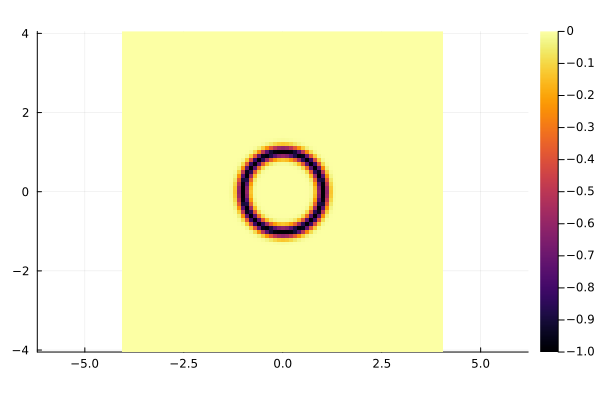
\includegraphics[width=0.3\textwidth]{circle.png}
\caption{\label{fig:frog}heatmap of intensity distribution of circle of radius 1}
\end{figure}

\subsection{Rotated Ellipse}
Equation for rotated Ellipse:
\begin{equation}
    \dfrac {((x-x_{0})\cos(\theta)+(y-y_{0})\sin(\theta))^2}{(R_x)^2}+\dfrac{((x-x_{0}) \sin(\theta)-(y-y_{0}) \cos(\theta))^2}{(R_y)^2}=1
\end{equation}
This equation can be parameterized using the angle $\alpha$ in the following way:
\begin{equation}
    \begin{aligned}
            x(\alpha) &= R_x \cos(\alpha) \cos(\theta) - R_y \sin(\alpha) \sin(\theta) + x_{0} \\
y(\alpha) &= R_x \cos(\alpha) \sin(\theta) + R_y \sin(\alpha) \cos(\theta) + y_{0}
    \end{aligned}
\end{equation}
Using a similar approach to the section above we can write:
\begin{equation}
    I(x,y)=A\exp\left({-(1-\sqrt{\dfrac {((x-x_{0})\cos(\theta)+(y-y_{0})\sin(\theta))^2}{(R_x)^2}+\dfrac{((x-x_{0}) \sin(\theta)-(y-y_{0}) \cos(\theta))^2}{(R_y)^2}})^{2}/\sigma^{2}}\right)
\end{equation}
\begin{figure}
\centering
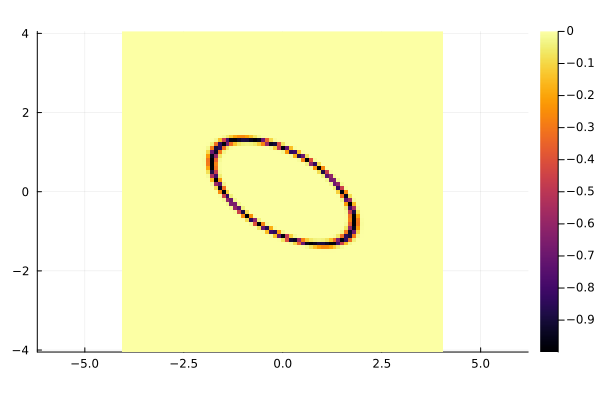
\includegraphics[width=0.3\textwidth]{ellipse.png}
\caption{\label{fig:ellipse}heatmap of intensity distribution of ellipse of $r_{x}=1$, $r_{y}=2$ and $\theta=\pi/3$}
\end{figure}


\end{document}